\documentclass{standalone}
\usepackage{tikz}
\usetikzlibrary{patterns, positioning}


\begin{document}
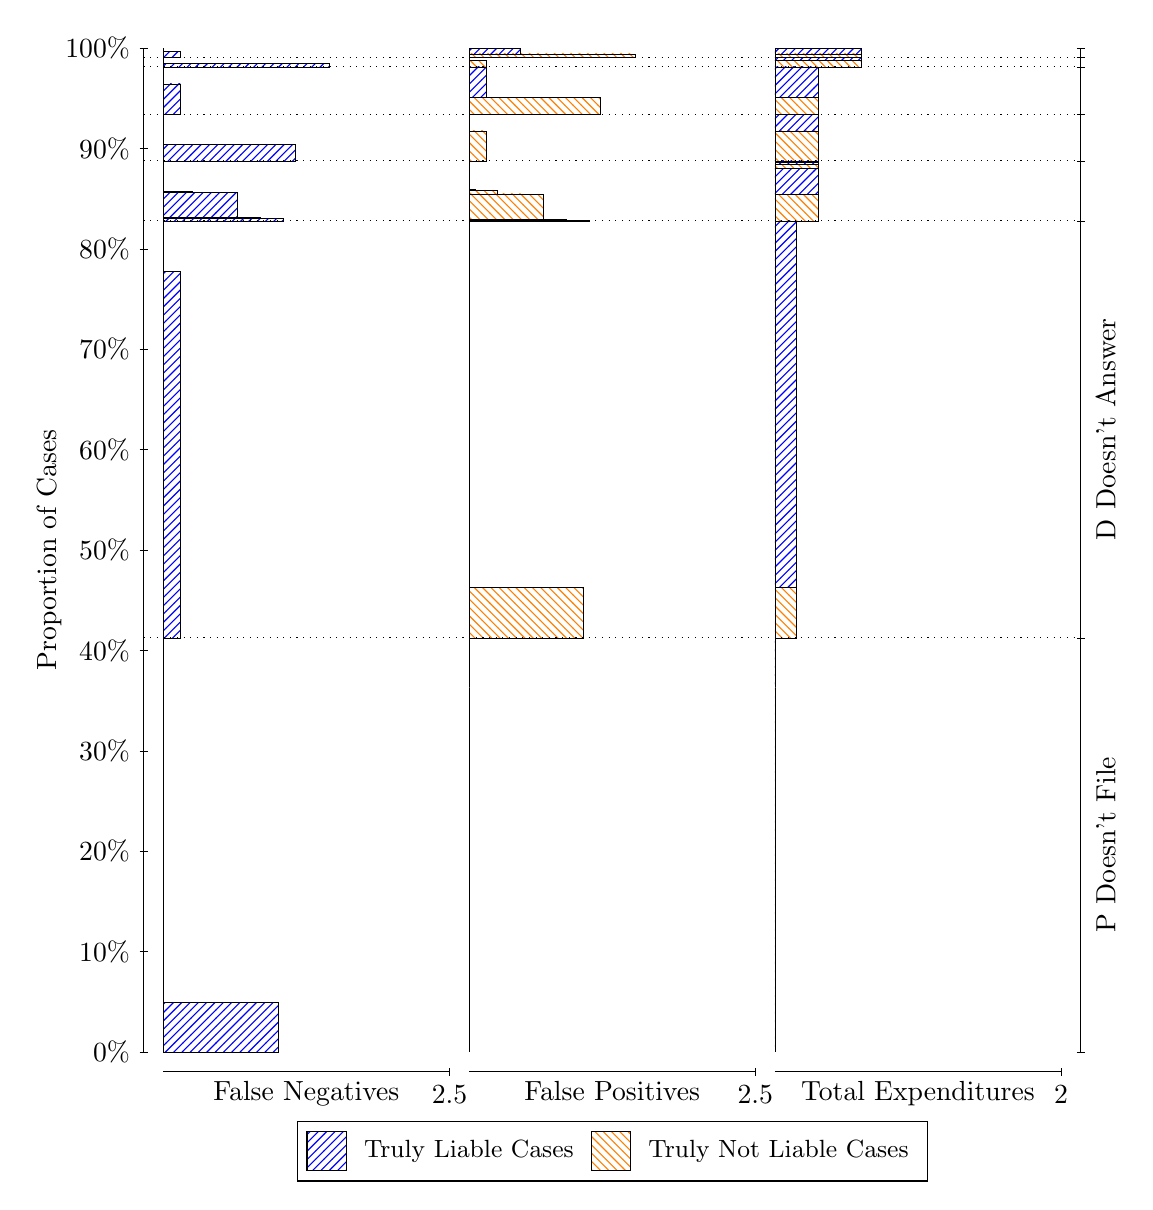
\begin{tikzpicture}
\draw[black, very thin] (1.5,1.75) -- (1.5,14.5);
\node[rotate=90, text=black, anchor=center] at (0.3, 8.125) {Proportion of Cases};
\draw[black, very thin] (1.45,1.75) -- (1.55,1.75);
\node[text=black, anchor=east] at (1.45, 1.75) {0\%};
\draw[black, very thin] (1.45,3.025) -- (1.55,3.025);
\node[text=black, anchor=east] at (1.45, 3.025) {10\%};
\draw[black, very thin] (1.45,4.3) -- (1.55,4.3);
\node[text=black, anchor=east] at (1.45, 4.3) {20\%};
\draw[black, very thin] (1.45,5.575) -- (1.55,5.575);
\node[text=black, anchor=east] at (1.45, 5.575) {30\%};
\draw[black, very thin] (1.45,6.85) -- (1.55,6.85);
\node[text=black, anchor=east] at (1.45, 6.85) {40\%};
\draw[black, very thin] (1.45,8.125) -- (1.55,8.125);
\node[text=black, anchor=east] at (1.45, 8.125) {50\%};
\draw[black, very thin] (1.45,9.4) -- (1.55,9.4);
\node[text=black, anchor=east] at (1.45, 9.4) {60\%};
\draw[black, very thin] (1.45,10.675) -- (1.55,10.675);
\node[text=black, anchor=east] at (1.45, 10.675) {70\%};
\draw[black, very thin] (1.45,11.95) -- (1.55,11.95);
\node[text=black, anchor=east] at (1.45, 11.95) {80\%};
\draw[black, very thin] (1.45,13.225) -- (1.55,13.225);
\node[text=black, anchor=east] at (1.45, 13.225) {90\%};
\draw[black, very thin] (1.45,14.5) -- (1.55,14.5);
\node[text=black, anchor=east] at (1.45, 14.5) {100\%};

\draw[black, very thin] (13.4,1.75) -- (13.4,14.5);
\draw[black, very thin] (13.35,1.75) -- (13.45,1.75);
\node[anchor=west] at (13.35, 1.75) {};
\draw[black, very thin] (13.35,7.01) -- (13.45,7.01);
\node[anchor=west] at (13.35, 7.01) {};
\draw[black, very thin] (13.35,12.306) -- (13.45,12.306);
\node[anchor=west] at (13.35, 12.306) {};
\draw[black, very thin] (13.35,13.067) -- (13.45,13.067);
\node[anchor=west] at (13.35, 13.067) {};
\draw[black, very thin] (13.35,13.659) -- (13.45,13.659);
\node[anchor=west] at (13.35, 13.659) {};
\draw[black, very thin] (13.35,14.261) -- (13.45,14.261);
\node[anchor=west] at (13.35, 14.261) {};
\draw[black, very thin] (13.35,14.383) -- (13.45,14.383);
\node[anchor=west] at (13.35, 14.383) {};
\draw[black, very thin] (13.35,14.5) -- (13.45,14.5);
\node[anchor=west] at (13.35, 14.5) {};

\draw[black, very thin, pattern color=blue, pattern=north east lines] (1.75,1.75) rectangle (3.2033,2.3828);
\draw[black, very thin, pattern color=orange, pattern=north west lines] (1.75,2.3828) rectangle (1.75,7.01);
\draw[black, very thin, pattern color=blue, pattern=north east lines] (1.75,7.01) rectangle (1.968,11.662);
\draw[black, very thin, pattern color=orange, pattern=north west lines] (1.75,11.662) rectangle (1.75,12.306);
\draw[black, very thin, pattern color=blue, pattern=north east lines] (1.75,12.306) rectangle (3.276,12.336);
\draw[black, very thin, pattern color=blue, pattern=north east lines] (1.75,12.336) rectangle (2.9853,12.345);
\draw[black, very thin, pattern color=blue, pattern=north east lines] (1.75,12.345) rectangle (2.6947,12.662);
\draw[black, very thin, pattern color=blue, pattern=north east lines] (1.75,12.662) rectangle (2.404,12.671);
\draw[black, very thin, pattern color=blue, pattern=north east lines] (1.75,12.671) rectangle (2.1133,12.682);
\draw[black, very thin, pattern color=orange, pattern=north west lines] (1.75,12.682) rectangle (1.75,13.067);
\draw[black, very thin, pattern color=blue, pattern=north east lines] (1.75,13.067) rectangle (3.4213,13.278);
\draw[black, very thin, pattern color=orange, pattern=north west lines] (1.75,13.278) rectangle (1.75,13.659);
\draw[black, very thin, pattern color=blue, pattern=north east lines] (1.75,13.659) rectangle (1.968,14.044);
\draw[black, very thin, pattern color=orange, pattern=north west lines] (1.75,14.044) rectangle (1.75,14.261);
\draw[black, very thin, pattern color=blue, pattern=north east lines] (1.75,14.261) rectangle (3.8573,14.305);
\draw[black, very thin, pattern color=orange, pattern=north west lines] (1.75,14.305) rectangle (1.75,14.383);
\draw[black, very thin, pattern color=blue, pattern=north east lines] (1.75,14.383) rectangle (1.968,14.457);
\draw[black, very thin, pattern color=orange, pattern=north west lines] (1.75,14.457) rectangle (1.75,14.5);
\draw[black, very thin, pattern color=orange, pattern=north west lines] (5.6333,1.75) rectangle (5.6333,6.3773);
\draw[black, very thin, pattern color=blue, pattern=north east lines] (5.6333,6.3773) rectangle (5.6333,7.01);
\draw[black, very thin, pattern color=orange, pattern=north west lines] (5.6333,7.01) rectangle (7.0867,7.6548);
\draw[black, very thin, pattern color=blue, pattern=north east lines] (5.6333,7.6548) rectangle (5.6333,12.306);
\draw[black, very thin, pattern color=orange, pattern=north west lines] (5.6333,12.306) rectangle (7.1593,12.313);
\draw[black, very thin, pattern color=orange, pattern=north west lines] (5.6333,12.313) rectangle (6.8687,12.322);
\draw[black, very thin, pattern color=orange, pattern=north west lines] (5.6333,12.322) rectangle (6.578,12.639);
\draw[black, very thin, pattern color=orange, pattern=north west lines] (5.6333,12.639) rectangle (6.2873,12.648);
\draw[black, very thin, pattern color=orange, pattern=north west lines] (5.6333,12.648) rectangle (5.9967,12.691);
\draw[black, very thin, pattern color=blue, pattern=north east lines] (5.6333,12.691) rectangle (5.706,12.702);
\draw[black, very thin, pattern color=blue, pattern=north east lines] (5.6333,12.702) rectangle (5.6333,13.067);
\draw[black, very thin, pattern color=orange, pattern=north west lines] (5.6333,13.067) rectangle (5.8513,13.447);
\draw[black, very thin, pattern color=blue, pattern=north east lines] (5.6333,13.447) rectangle (5.6333,13.659);
\draw[black, very thin, pattern color=orange, pattern=north west lines] (5.6333,13.659) rectangle (7.3047,13.875);
\draw[black, very thin, pattern color=blue, pattern=north east lines] (5.6333,13.875) rectangle (5.8513,14.261);
\draw[black, very thin, pattern color=orange, pattern=north west lines] (5.6333,14.261) rectangle (5.8513,14.34);
\draw[black, very thin, pattern color=blue, pattern=north east lines] (5.6333,14.34) rectangle (5.6333,14.383);
\draw[black, very thin, pattern color=orange, pattern=north west lines] (5.6333,14.383) rectangle (7.7407,14.426);
\draw[black, very thin, pattern color=blue, pattern=north east lines] (5.6333,14.426) rectangle (6.2873,14.5);
\draw[black, very thin, pattern color=orange, pattern=north west lines] (9.5167,1.75) rectangle (9.5167,6.3773);
\draw[black, very thin, pattern color=blue, pattern=north east lines] (9.5167,6.3773) rectangle (9.5167,7.01);
\draw[black, very thin, pattern color=orange, pattern=north west lines] (9.5167,7.01) rectangle (9.7892,7.6548);
\draw[black, very thin, pattern color=blue, pattern=north east lines] (9.5167,7.6548) rectangle (9.7892,12.306);
\draw[black, very thin, pattern color=orange, pattern=north west lines] (9.5167,12.306) rectangle (10.062,12.639);
\draw[black, very thin, pattern color=blue, pattern=north east lines] (9.5167,12.639) rectangle (10.062,12.976);
\draw[black, very thin, pattern color=orange, pattern=north west lines] (9.5167,12.976) rectangle (10.062,13.019);
\draw[black, very thin, pattern color=blue, pattern=north east lines] (9.5167,13.019) rectangle (10.062,13.049);
\draw[black, very thin, pattern color=orange, pattern=north west lines] (9.5167,13.049) rectangle (10.062,13.058);
\draw[black, very thin, pattern color=blue, pattern=north east lines] (9.5167,13.058) rectangle (10.062,13.067);
\draw[black, very thin, pattern color=orange, pattern=north west lines] (9.5167,13.067) rectangle (10.062,13.447);
\draw[black, very thin, pattern color=blue, pattern=north east lines] (9.5167,13.447) rectangle (10.062,13.659);
\draw[black, very thin, pattern color=orange, pattern=north west lines] (9.5167,13.659) rectangle (10.062,13.875);
\draw[black, very thin, pattern color=blue, pattern=north east lines] (9.5167,13.875) rectangle (10.062,14.261);
\draw[black, very thin, pattern color=orange, pattern=north west lines] (9.5167,14.261) rectangle (10.607,14.34);
\draw[black, very thin, pattern color=blue, pattern=north east lines] (9.5167,14.34) rectangle (10.607,14.383);
\draw[black, very thin, pattern color=orange, pattern=north west lines] (9.5167,14.383) rectangle (10.607,14.426);
\draw[black, very thin, pattern color=blue, pattern=north east lines] (9.5167,14.426) rectangle (10.607,14.5);
\draw[black, dotted] (1.5,7.01) -- (13.4,7.01);
\draw[black, dotted] (1.5,12.306) -- (13.4,12.306);
\draw[black, dotted] (1.5,13.067) -- (13.4,13.067);
\draw[black, dotted] (1.5,13.659) -- (13.4,13.659);
\draw[black, dotted] (1.5,14.261) -- (13.4,14.261);
\draw[black, dotted] (1.5,14.383) -- (13.4,14.383);
\draw[black, very thin] (1.75,1.5) -- (5.3833,1.5);
\node[text=black, anchor=north] at (3.5667, 1.5) {False Negatives};
\draw[black, very thin] (5.3833,1.45) -- (5.3833,1.55);
\node[text=black, anchor=north] at (5.3833, 1.45) {2.5};

\draw[black, very thin] (5.6333,1.5) -- (9.2667,1.5);
\node[text=black, anchor=north] at (7.45, 1.5) {False Positives};
\draw[black, very thin] (9.2667,1.45) -- (9.2667,1.55);
\node[text=black, anchor=north] at (9.2667, 1.45) {2.5};

\draw[black, very thin] (9.5167,1.5) -- (13.15,1.5);
\node[text=black, anchor=north] at (11.333, 1.5) {Total Expenditures};
\draw[black, very thin] (13.15,1.45) -- (13.15,1.55);
\node[text=black, anchor=north] at (13.15, 1.45) {2};

\node[text=black, centered, rotate=90] at (13.72, 4.38) {P Doesn't File};
\node[text=black, centered, rotate=90] at (13.72, 9.6582) {D Doesn't Answer};






\draw (7.449999999999999,1.5) node[draw=none] (baseCoordinate) {};
\begin{scope}[align=center]
        \matrix[scale=0.5, draw=black, below=0.5cm of baseCoordinate, nodes={draw}, column sep=0.1cm]{
            \node[rectangle, draw, minimum width=0.5cm, minimum height=0.5cm, pattern color=blue, pattern=north east lines] {}; &
            \node[draw=none, font=\small, text=black] (B) {Truly Liable Cases}; &
            \node[rectangle, draw, minimum width=0.5cm, minimum height=0.5cm, pattern color=orange, pattern=north west lines] {}; &
            \node[draw=none, font=\small, text=black] (B) {Truly Not Liable Cases}; \\
            };
\end{scope}

\end{tikzpicture}
\end{document}